La figure suivante représente l'onde observée lorsque le signal possède une fréquence d'1MHz et qu'un des fils est resté en circuit ouvert. (voir \ref{fig:Signal à 1MHz}) La
ligne bleu représente le signal à l'entrée du circuit (connecteur du fil A). La ligne jaune représente le signal à l'extrémité du circuit
(connecteur du fil B).

\begin{figure}[H]
    \centering
    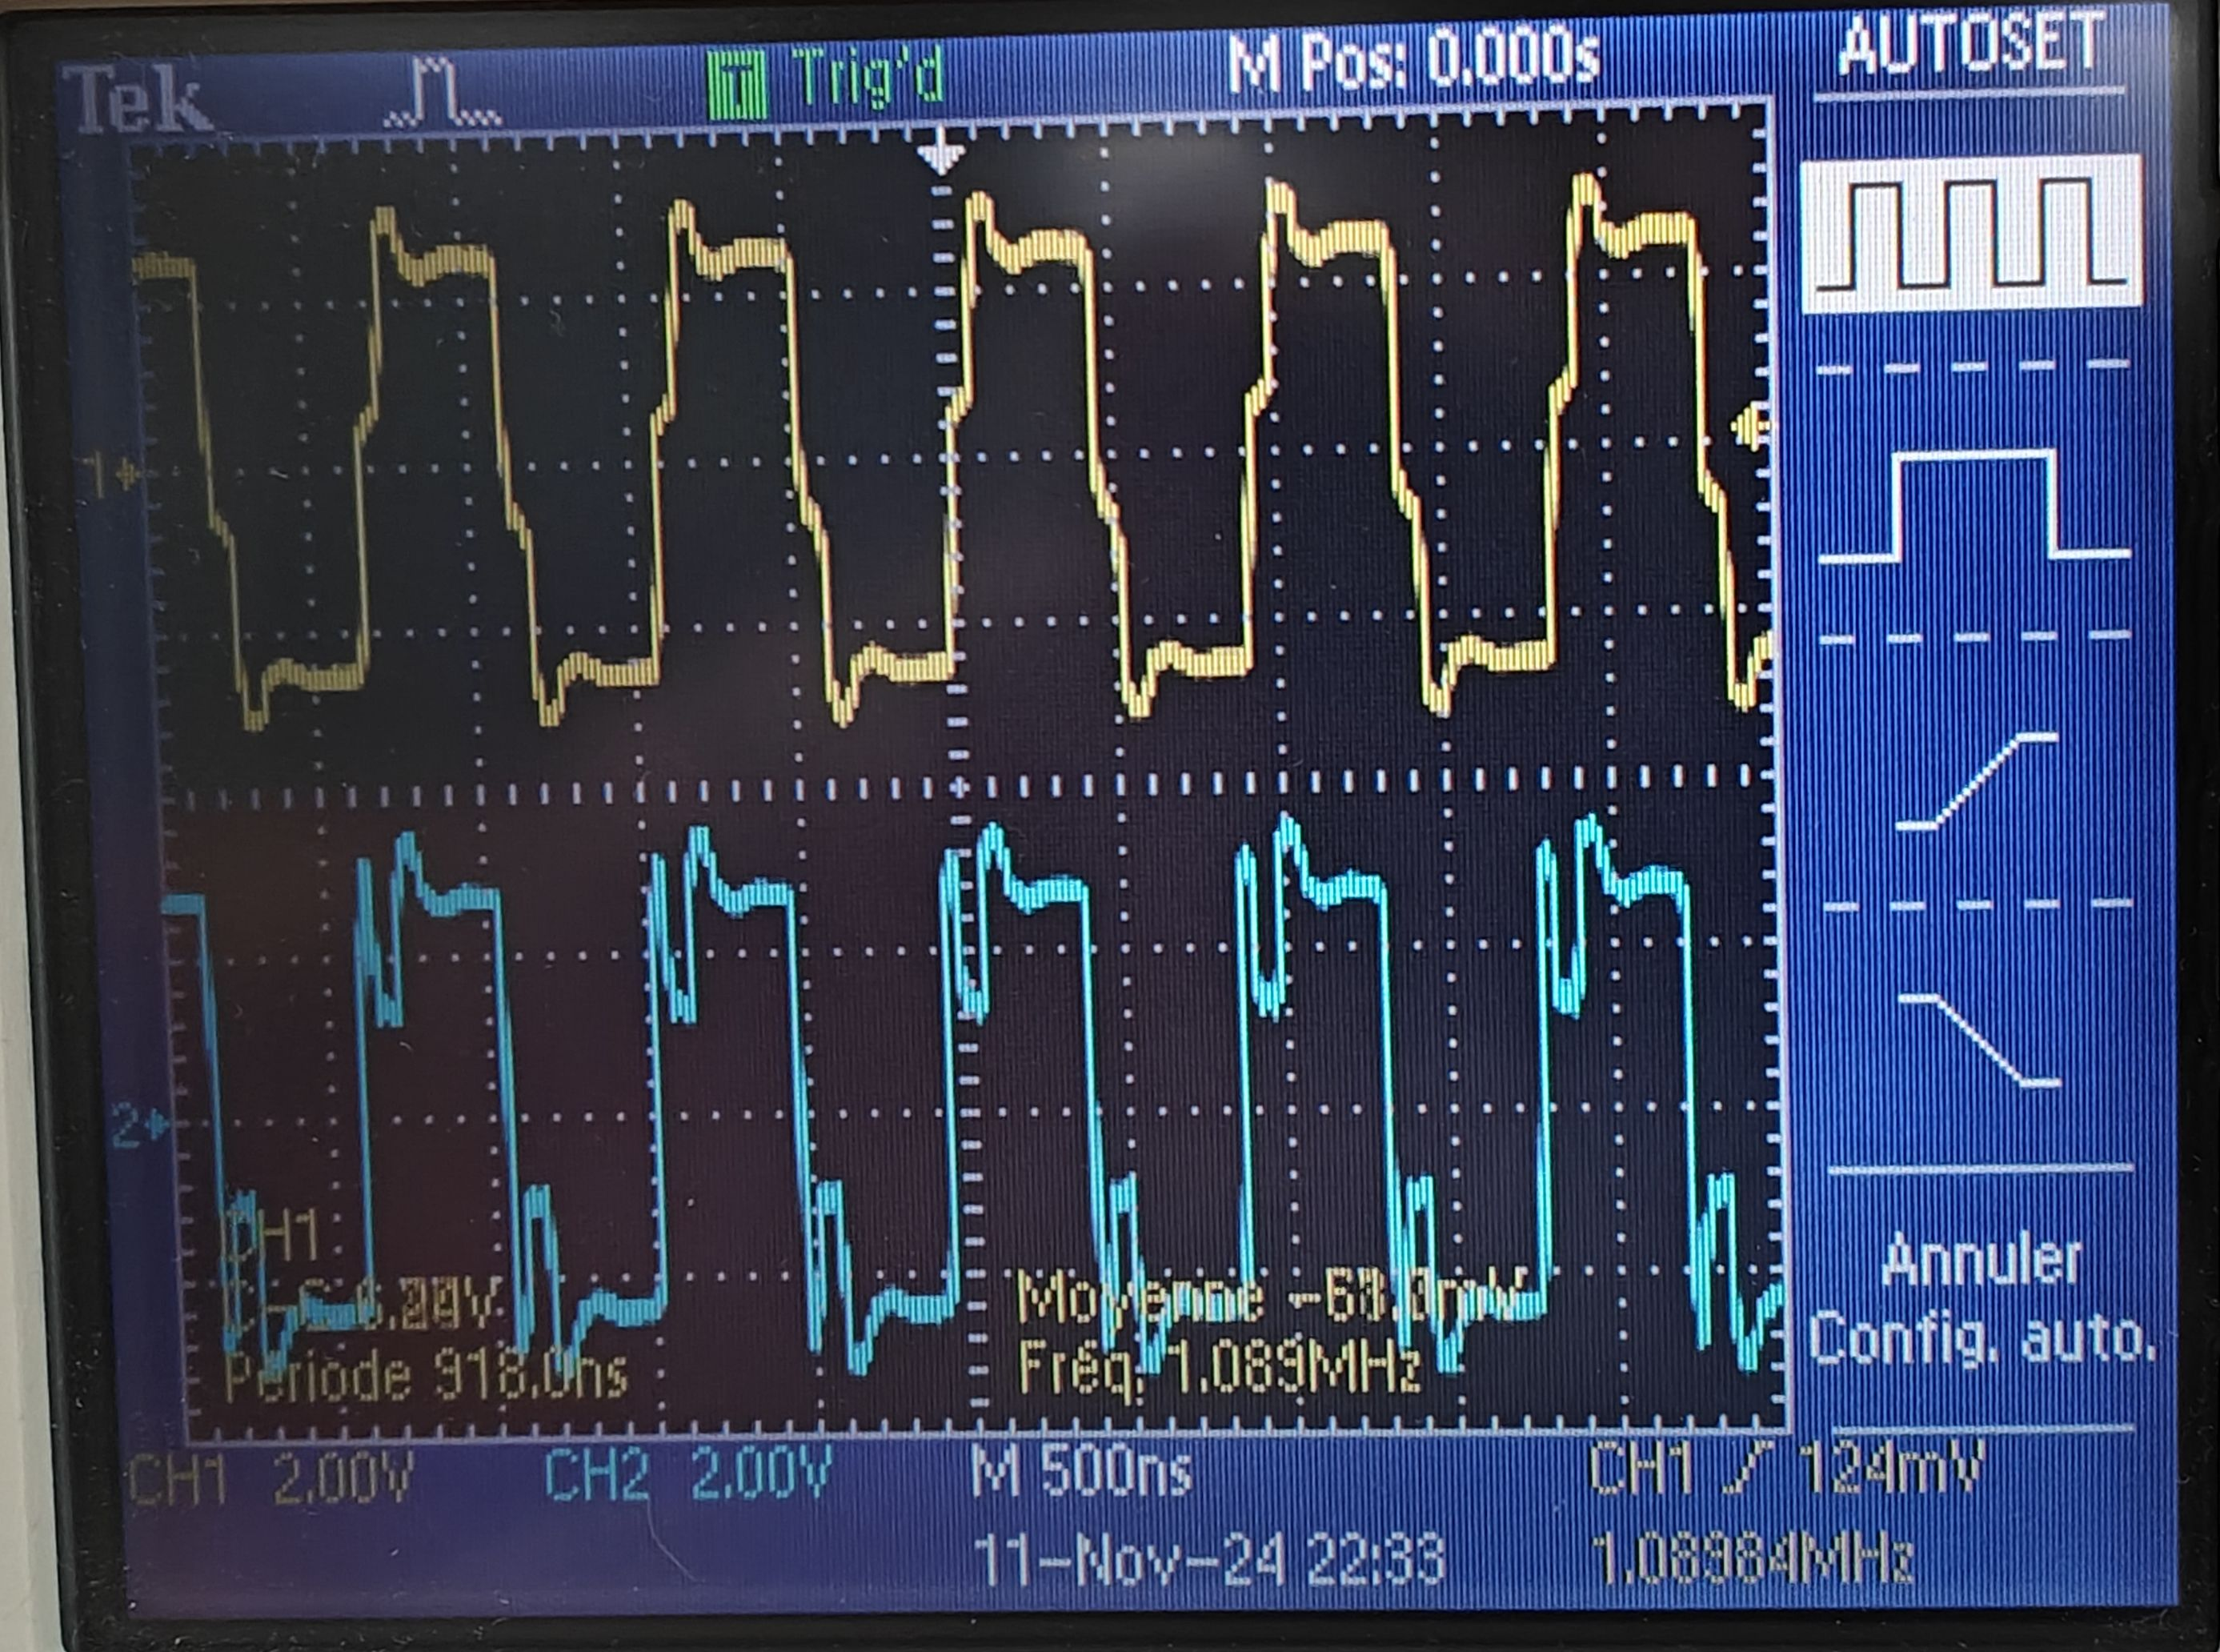
\includegraphics[width=0.7\textwidth]{images/1mhz.jpg}
    \caption{Signaux d'entrée et de sortie à 1MHz}
    \label{fig:Signal à 1MHz}
\end{figure}

On peux voir que les impulsions carrées sont déformées par la réflexion du signal sur la branche ouverte. La réflexion est aussi forte car lorsqu'un fil est laissé en circuit ouvert, sont impédance est infinie. Par contre, les impulsions ont une amplitude de plus de 2V et une durée d'environ 450ns ce qui est adéquat pour que la carte réseau les décode correctement.
